\documentclass[journal, onecolumn]{IEEEtran}

\ifCLASSOPTIONcompsoc
  % IEEE Computer Society needs nocompress option
  % requires cite.sty v4.0 or later (November 2003)
  \usepackage[nocompress]{cite}
\else
  % normal IEEE
  \usepackage{cite}
\fi

% All pdf figures are stored in this folder
\usepackage[pdftex]{graphicx}
\usepackage[T1]{fontenc}
\usepackage{array}
\usepackage[justification=centering]{caption}
%\usepackage{hyperref}
\graphicspath{{./figures/}}

\newcommand\uml[1]{\texttt{\textbf{#1}}}
\newcommand\cg[1]{\textit{#1}}
%\usepackage{xcolor}
%\usepackage{colortbl}
\usepackage{xcolor,colortbl}
\definecolor{Gray}{gray}{0.85}
% *** GRAPHICS RELATED PACKAGES ***
%
\ifCLASSINFOpdf
  % \usepackage[pdftex]{graphicx}
  % declare the path(s) where your graphic files are
  % \graphicspath{{../pdf/}{../jpeg/}}
  % and their extensions so you won't have to specify these with
  % every instance of \includegraphics
  % \DeclareGraphicsExtensions{.pdf,.jpeg,.png}
\else
  % or other class option (dvipsone, dvipdf, if not using dvips). graphicx
  % will default to the driver specified in the system graphics.cfg if no
  % driver is specified.
  % \usepackage[dvips]{graphicx}
  % declare the path(s) where your graphic files are
  % \graphicspath{{../eps/}}
  % and their extensions so you won't have to specify these with
  % every instance of \includegraphics
  % \DeclareGraphicsExtensions{.eps}
\fi

\hyphenation{op-tical net-works semi-conduc-tor}

\begin{document}
%
% paper title
% Titles are generally capitalized except for words such as a, an, and, as,
% at, but, by, for, in, nor, of, on, or, the, to and up, which are usually
% not capitalized unless they are the first or last word of the title.
% Linebreaks \\ can be used within to get better formatting as desired.
% Do not put math or special symbols in the title.
\title{When Asteroids Attack: The MWSU Simulation Team's Adventure in High Level Architecture and Distributed Simulation}
% author names and affiliations
% use a multiple column layout for up to three different
% affiliations

% conference papers do not typically use \thanks and this command
% is locked out in conference mode. If really needed, such as for
% the acknowledgment of grants, issue a \IEEEoverridecommandlockouts
% after \documentclass

% for over three affiliations, or if they all won't fit within the width
% of the page (and note that there is less available width in this regard for
% compsoc conferences compared to traditional conferences), use this
% alternative format:
%

\author{\IEEEauthorblockN{Bingyang Wei\IEEEauthorrefmark{1},
Amy Knowles, Christopher Silva, Christine Mounce} \\
\IEEEauthorblockA{Department of Computer Science \\
Midwestern State University, \\
Wichita Falls, Texas 76308\\ \IEEEauthorrefmark{1}Email: bingyang.wei@mwsu.edu}}

% make the title area
\maketitle

% As a general rule, do not put math, special symbols or citations
% in the abstract
\begin{abstract}
The Simulation Exploration Experience (SEE) is an annual, inter-university, distributed simulation challenge led by NASA. A primary objective is to provide a platform for college students to work in highly dispersed teams to design, develop, test, and execute a simulated lunar mission using High Level Architecture. During the SEE in 2016, 19 federates developed by student teams from three continents successfully joined the HLA federation and collaborated to accomplish a lunar mission. The Midwestern State University team first participated in SEE 2016 by developing a communication satellite federate which broadcast an alert about the incoming of an asteroid to physical entities on the surface of the moon. This paper describes SEE, High Level Architecture, the NASA and other team federates, the MWSU Sim Team experience, lessons learned and recommendations for future teams.
\end{abstract}

% For peer review papers, you can put extra information on the cover
% page as needed:
% \ifCLASSOPTIONpeerreview
% \begin{center} \bfseries EDICS Category: 3-BBND \end{center}
% \fi
%
% For peerreview papers, this IEEEtran command inserts a page break and
% creates the second title. It will be ignored for other modes.
\IEEEpeerreviewmaketitle

\section{Introduction}
Modeling and Simulation (M\&S) is the representation of the behavior or characteristics of one system, such as the moon, through the use of another system, which in our case is a diverse group of computer programs designed under the High Level Architecture (HLA) standard. Simulations allow us to view and explore the behavior of a system that may be too expensive or too risky to explore in the real world. Interest in M\&S has increased greatly over recent years, in part due to the following reasons:
\begin{itemize}
	\item Simulations are generally less expensive, and far safer than real-world experiments (ex. supercomputer simulations of nuclear explosions)
	\item Simulations can be more immersive than attempts at real-world experiments (ex. simulations of surface conditions of nearby planets in 
		preparation for future NASA missions)
	\item Simulations can be performed faster than real-time (ex. weather simulations)
\end{itemize}

Although interest in M\&S has greatly increased over recent years, there is still a lack of undergraduate level programs focusing on the design and implementation of simulation.  As M\&S is quickly becoming a multi-billion dollar industry, a highly skilled workforce is required.  In order to develop this workforce, modeling and simulation programs need to be developed starting in public school and ranging all the way through graduate level studies.  Although programs exist at the masters level and above, few programs exist at the undergraduate level \cite{banks2008compelling}.  The SEE program is an excellent introduction to distributed simulation as it provides faculty advisors and students with the needed elements: content, software, tools, systems, mentoring, along with project management support in an attempt to expand M\&S undergraduate level education.

Initiated in 2011, the annual Simulation Exploration Experience event, formally known as SISO Smackdown, has successfully promoted the awareness of the use of High Level Architecture (HLA) in distributed simulation around the world. During the event, academia, industry and professional associations collaborate to design, develop, test and demonstrate a simulated lunar mission. SEE provides an excellent platform for college students to learn and practice both M\&S and software engineering concepts and principles. More importantly, the opportunity of working closely with M\&S professionals in industry and associations is an invaluable experience to the students. 

SEE originated with NASA engineer Zack crues and has been implemented annualy since 2011 by NASA and the SISO Space Community Forum.  It was developed as a way engage students in modeling and simulation, an area of education almost non-existant at the undergraduate level.  Because SEE involves geographically distributed inter-university teams, it proves to the participants that interoperability and standards matter in order to allow distributed parts of the simulation to work seamlessly. This program allows students to learn HLA in a fail-free environment with expert and peer support, to learn employer expectations first-hand, as well as allow them to assess their interest and aptitude for a career in M\&S.  

This paper concentrates on the learning experience of Midwestern State University team members, their interactions with other student teams across the world, industry representatives from Pitch, and NASA engineers at both JSC and KSC.  The rest of the paper is structured as follows: Section II provides an introduction to High Level Architecture (HLA); Section III describes in detail the 2016 experience of the Midwestern State University (MWSU) team; Lessons learned from SEE are discussed in Section IV and Section V concludes the paper and provides instructions for future teams to join SEE.

\section{High Level Architecture}
High-Level Architecture(HLA) is an architecture that allows many distributed simulation systems to work together seamlessly. \\
		There are five parts to a HLA system:
		\begin{itemize}
			\item Runtime Infrastructure(RTI) - Software that provides HLA services.
			\item Federate - A simulation system that connects to the RTI.
			\item Federation Object Model(FOM) - A description of data exchanges in a federation.
			\item Federation - All of the federates along with the RTI and the FOM they use.
			\item Federation Execution - An instance of the federation.
		\end{itemize}
		HLA uses a publish/subscribe methodology for information services. This means that a federate "publishes" certain data and "subscribes" to other data. To publish data a federate sends it to the RTI. To receive subscribed data a federate will receive a callback from the RTI anytime the subscribed data is updated. \\
%\begin{figure}[!htbp]
%	\centering
%		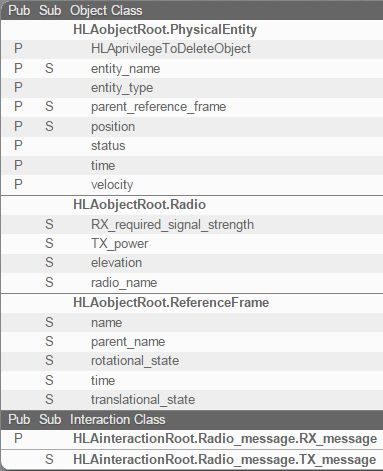
\includegraphics[width=\linewidth]{interactions.png}
%		\caption{MWSU Satellite publish/subscribe listing.}
%	\label{interactions}
%\end{figure}
		
		The FOM contains descriptions of the Objects, Interactions, and Data Types that federates will use in a federation. Because of this all federates must agree on which FOMs to use. This is arguably the most important part of the HLA standard; it ensures that the designers of each federate communicate in order to come to an agreement on not just the FOM, but on other aspects such as the overall goal of the simulation.
%\begin{figure}[!htbp]
%	\centering
%		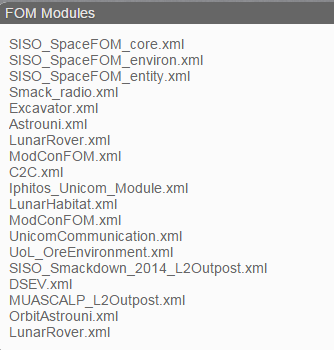
\includegraphics[width=\linewidth]{fom.png}
%		\caption{FOMs used in SEE 2016.}
%	\label{fom}
%\end{figure}		
		
The recommended representation for a federation is called a "lollipop" diagram (see Figure \ref{lollipop}). 
\begin{figure}[!htbp]
	\centering
		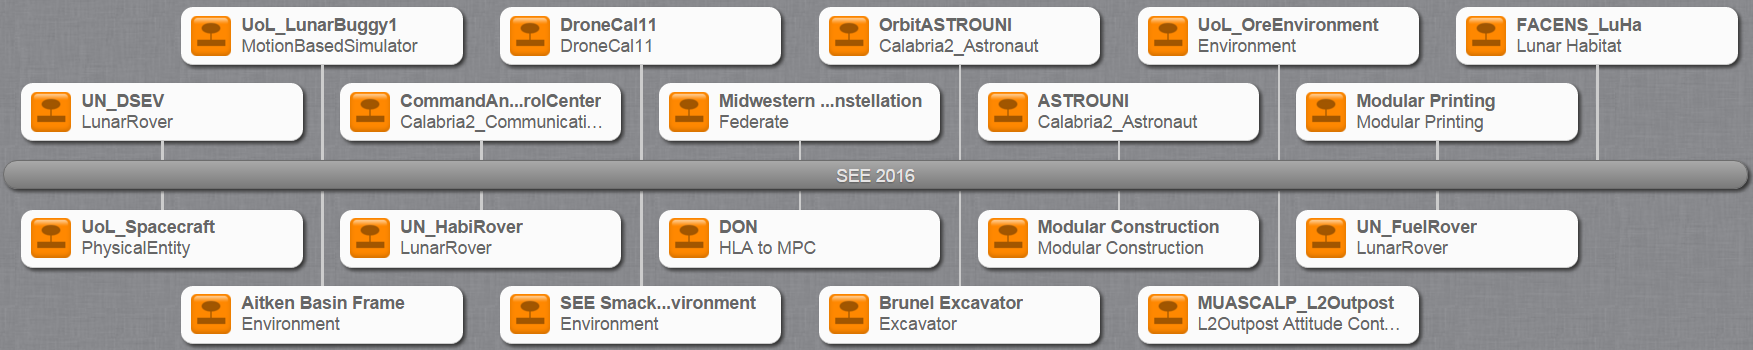
\includegraphics[width=\linewidth]{lollipop.png}
		\caption{SEE 2016 participants lollipop diagram.}
	\label{lollipop}
\end{figure}		
\section{2016 SEE Experience}
The Simulation Exploration Experience, hosted by NASA was an exciting and immersive experience in modeling and distributed simulation.  The 2016 MWSU Sim team consisted of four computer science students, one graduate and three undergraduates, and our sponsoring professor and local HLA expert, Dr. Wei.  We began meeting formally late in the Fall 2015 semester in preparation for our participation in the SEE 2016 workshop at the 2016 SCS Spring Simulation Multi-Conference (SpringSim '16) that took place in Liverpool, England.  This experience allowed us to implement knowledge learned in multiple courses, such as software engineering, discrete system simulation, and contemporary programming.

Our first step in preparing ourselves for writing our own federate was to download the HLA tutorial available on the Pitch website\cite{HLA}.  Once we fully understood the HLA model, we were able to access and complete numerous tutorials on creating federates available to participating SEE team members in the SEE Assembla repository. The following subsections describe the MWSU Sim team satellite federate, and the team's experiences interacting with industry professions, NASA engineers, and college students from around the world.

\subsection{Satellite Constellation \& Lunar Visualization Module}
The Satellite Constellation \& Lunar Visualization module first propagates and then renders satellite constellations. STK\rq{}s numerical propagator is invoked to generate the orbits of different satellites. The constellation is achieved by STK\rq{}s High Precision Orbit Propagator (HPOP) which is a part of the Orbit Propagation Library (OPL). By numerically integrating the various forces affecting satellites, HPOP brings high fidelity orbit propagation into our MWSU communication satellites.

When the whole federation is running on Pitch RTI, a 6-satellite constellation is designed over Aitken Basin to maximize the time each satellite is in view of the surface entities as shown in Figure \ref{Satellites}.
\begin{figure}[!htbp]
	\centering
		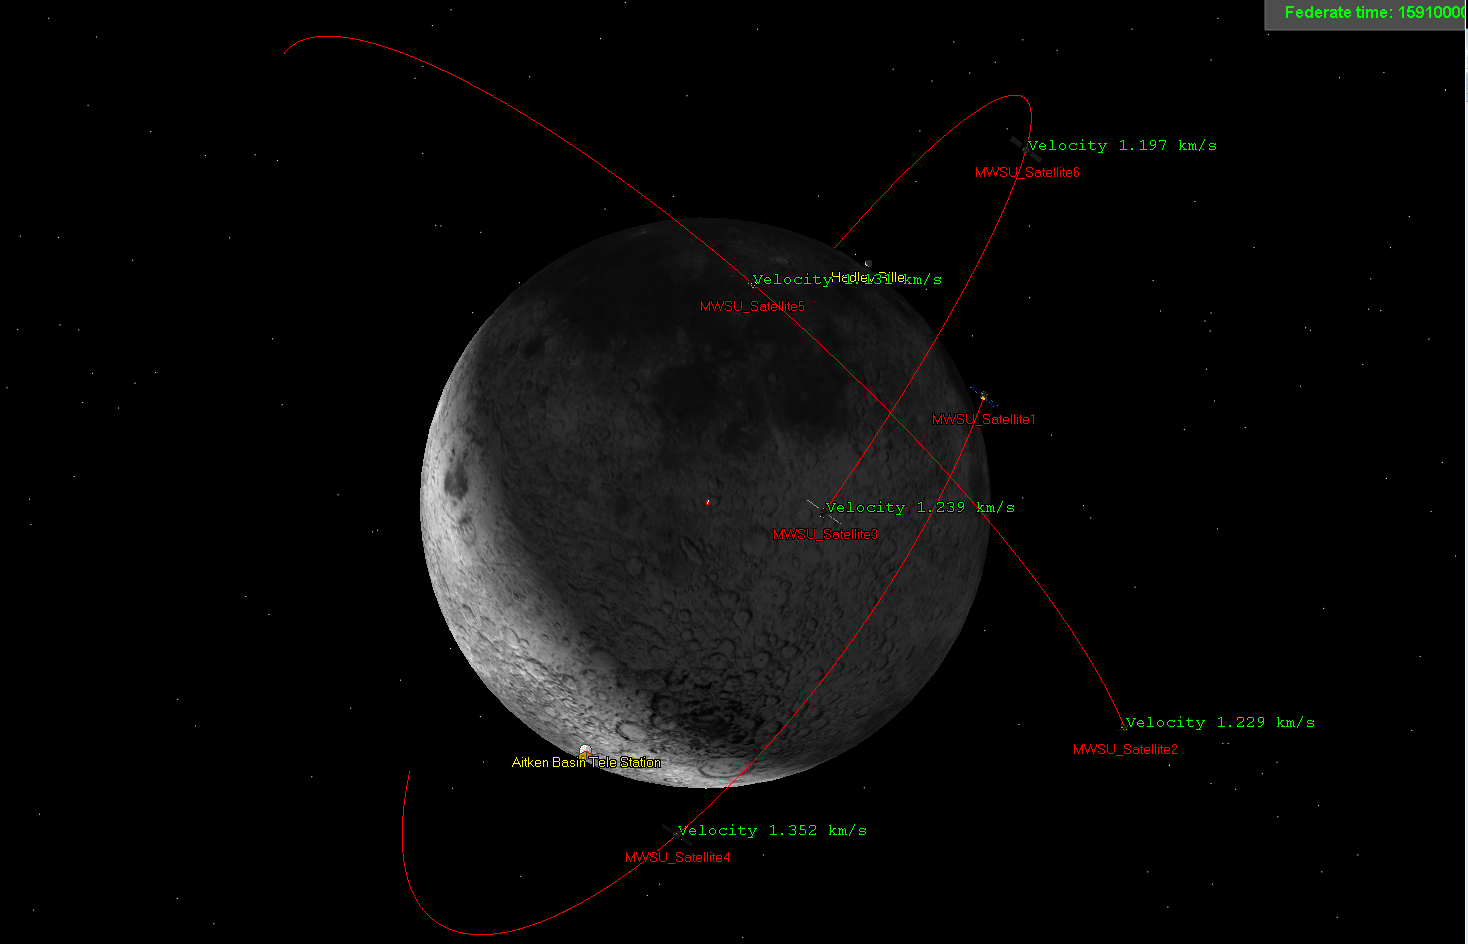
\includegraphics[width=100mm]{Satellites.PNG}
		\caption{MWSU communication satellites federate.}
	\label{Satellites}
\end{figure}

The architecture of the Satellite Constellation \& Lunar Visualization module is shown in, Figure \ref {Class}, a UML class diagram.

\begin{figure}[!htbp]
	\centering
		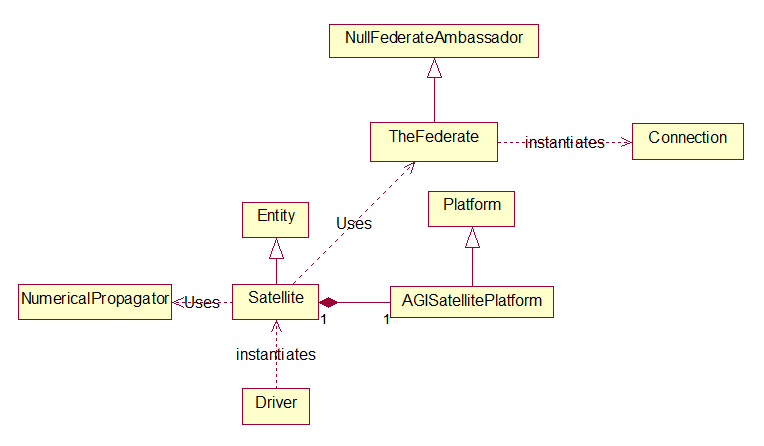
\includegraphics[width=100mm]{ClassDiagram.png}
		\caption{MWSU satellite constellation \& lunar visualization module class diagram.}
	\label{Class}
\end{figure}

\subsection{\textit{Tag Ups} \& SpringSim '16}
Starting in November 2015, the MWSU Sim team participated in weekly \textit{tag ups} which occurred at 09:00 CST (06:00 UTC) every Wednesday.  These hour-long meetings utilized a software called VSEE, a visual telecommunication software, that allowed teams from universities around the world, representatives from Pitch and VT M{\"A}K, as well as NASA engineers at both Johnson Space Center(JSC) and Kennedy Space Center(KSC) to communicate and share their progress.  As March 2016 approached, the VSEE \textit{tag ups} were used for preliminary connection testing. During these testing \textit{tag ups}, the Pitch RTI was initiated, then the three NASA world origination federates were connected to the RTI.  Once the simulated world had been instantiated, each team was asked individually to attempt to connect their federate to the Pitch RTI.  Connection of the MWSU satellite federate to the Pitch RTI was performed by first connecting to the VPN, initializing our satellite federate, and upon request from the VSEE meeting organizer, connection to the Pitch RTI.  

The MWSU Sim team participated remotely, via VSEE, that took place at the 2016 SCS Spring Simulation Multi-Conference (SpringSim '16) in Liverpool, England.  During SEE 2016, a lunar mission was simulated. NASA JSC, KSC and 12 universities from three continents participated in this year\rq{}s distributed simulation event. All participants conformed to the IEEE HLA standard 1516-2010 for modeling and simulation. As usual, NASA provided basic support to the entire simulation mission, JSC regulated the time of the simulation while KSC provided real-time visualization of the simulation mission. Each university contributed to the lunar simulation by implementing a part of the entire simulation called a federate (More HLA terminologies are available in \cite{HLA}). A description of the SEE 2016 simulated mission follows: Astronauts explore a huge impact crater close to the south pole of the moon, called Aitken Basin.  Viewers are then introduced to a number of new lunar research units and construction sites: a 3D-printing site by University of Alberta (Canada), a supply depot, oxidizer and propellant production facility by University of Bordeaux (France), an astronaut habitat site by Facens (Brazil), a cargo rover by Florida Institute of Technology, a fuel rover by University of Nebraska, a lunar buggy and an unmanned aerial vehicle (UAV) by University of Liverpool (England).

The peaceful exploration operation is suddenly interrupted by the detection of an incoming asteroid by an asteroid detection system developed by University of Genoa (Italy). The command and communication center \cite{falcone2014simulation} developed by University of Calabria (Italy) alerts all physical entities on the surface of the moon, and the communication satellites developed by Midwestern State University alert the lunar buggy which is out of reach of the command and control center.

During the simulation, all nineteen federates connected successfully to the runtime infrastructure (RTI) provided by Pitch Technologies and were able to advance time (see Figure \ref{lollipop}). Each rectangle represents a joined federate and the middle gray bar denotes the RTI.

\section{Lessons Learned}
During the integration test and the final demo, we found several problems with our federate.  The MWSU federate was able to locate all physical entities in the Insight3D viewer, and verify the location and motion information of different entities in the orbit of the moon or on the surface.  

Although several problems with our federate were found during the integration testing, the only problem we were unable to fix was the M{\"A}K RTI exception:


Problem: MWSU federate worked well with Pitch RTI but failed to run on M{\"A}K RTI. When testing on M{\"A}K RTI, exception ``unsatisfiedLinkError makRtiJava1516e.dll: the specified procedure could not be found\rq\rq{} is thrown.
Solution: MWSU federate is a Java application built in Eclipse. This is an old problem with M{\"A}K RTI which does not work with the most recent version of the Java IDE. We attempted to downgrade our Java IDE environment/code in order to communicate with the M{\"A}K RTI, as suggested by members of the 2013 UAHuntsville team \cite{bulgatz2012design}. We were unable to solve this problem and have informed engineers at VT M{\"A}K. We hope this issue can be fixed for SEE 2017.

\section{Advice for Future Teams}
The more teams that participate in SEE, the better the experience for everyone involved.  If you would like to start a SEE Sim team at your university please visit the http://www.exploresim.com/team.\\
The requirements to start a team are:
\begin{enumerate}
	\item Minimum team must have at least one college faculty advisor and one student with knowledge of C++ and/or JAVA with the readiness to learn HLA 	 		Evolved, use standards and participate in an inter-university internationl simulation experience.  
	\item Teams can consist of a class, independent researchers, a departmental project, an interdepartmental project or inter-university undertaking.
	\item each team should have a team leader responsible for communication with the SEE Operations, Technical and Executive leaders and committees.
\end{enumerate}

The steps to start a team of your own are as follows:
\begin{enumerate}
	\item Read the requirements necessary to form a team (mentioned above).
	\item Fill out and submit teh team official interest form.
	\item Wait to be contacted by SEE General Manager Stephen Paglialonga.
\end{enumerate}

Once you have a team consisting of at least one faculty advisor and one student willing to learn HLA, in depth study of HLA should begin.  The best place to start is to read the HLA Tutorial available at http://www.pitchtechnologies.com/hlatutorial/.  It is our suggestion that a minimum of one month be given to the study of HLA in order to fully understand the infrastructure and intricacy of the system.  After everyone on the team has reached some degree of familiarity with the HLA infrastructure, and has acquired access to the SEE team development website, the Assembla Repository will be available.  This repository houses not only a fantastic interactive tutorial on creating a federate using Java, but also the Aitkin Basin and Environment federates developed by NASA engineer Zack Crues.  These two federates are the cornerstone of the entire lunar mission simulation and are extremely well-commented, making them one of the best learning tools available.
The next step is to decide what meaningful federate to build.  Does your team want to create a satellite system to relay information, a giant laser to target incoming asteroids, or a moon buggy to transport researchers around the lunar base?  Creating a meaningful federate that will interact cooperatively with federates created by other inter-university teams is vital to the overall experience of SEE.  After your team has decided on an idea for a federate, the team needs to decide on application logic: how are you going to create this federate?  Are you going to use STK written in Java and Eclipse for visualization?  If you do, remember that the M{\"A}K RTI does not yet work well with Java applications.   Finally, the team needs to consider how to connect the federate to the federation, as the whole purpose of this exciting exercise is to work with other university students, professional engineers, and industry representatives to develop a distributed simulation.

% conference papers do not normally have an appendix

% trigger a \newpage just before the given reference
% number - used to balance the columns on the last page
% adjust value as needed - may need to be readjusted if
% the document is modified later
%\IEEEtriggeratref{8}
% The "triggered" command can be changed if desired:
%\IEEEtriggercmd{\enlargethispage{-5in}}

% references section

% can use a bibliography generated by BibTeX as a .bbl file
% BibTeX documentation can be easily obtained at:
% http://www.ctan.org/tex-archive/biblio/bibtex/contrib/doc/
% The IEEEtran BibTeX style support page is at:
% http://www.michaelshell.org/tex/ieeetran/bibtex/
\bibliographystyle{IEEEtran}
\bibliography{bibliography}
% argument is your BibTeX string definitions and bibliography database(s)
%\bibliography{IEEEabrv,../bib/paper}
%
% <OR> manually copy in the resultant .bbl file
% set second argument of \begin to the number of references
% (used to reserve space for the reference number labels box)

%\begin{thebibliography}{1}

%\bibitem{IEEEhowto:kopka}
%H.~Kopka and P.~W. Daly, \emph{A Guide to \LaTeX}, 3rd~ed.\hskip 1em plus
%  0.5em minus 0.4em\relax Harlow, England: Addison-Wesley, 1999.

%\end{thebibliography}




% that's all folks
\end{document}
